\chapter{Verification and Validation}\label{chapter:VV}
Verification and validation is arguably the most important step in any modeling process, since it reflects the accuracy of your numerical model. To that purpose, the take-off model is firstly verified by comparing to models found in literature. Afterwards, the model is validated using data found in FCOMs of several aircraft like the Dash8 and ATR72.

\section{Verification}\label{sec:verification}
Model verification is the process of comparing a numerical solution to theory. For take-off verification, several models exist which are described in \autoref{tab:verification_models}. Something that is unique to propeller take-off modeling is that the thrust cannot easily be averaged, which is possible for jet engines. Most models in literature assume jet engines are used and are thus thrust-based. However this is not correct for propeller since thrust will vary strongly with velocity for propellers. Therefore, it is important to appreciate what models use a thrust- or power-based approach. Furthermore, the models also vary in their $C_L$ definition and the number of flight phases.

\begin{table}[!ht]
    \centering
    \begin{tabular}{cccc} \hline
       \textbf{Model}       & \textbf{Method}   & $C_L$ \textbf{used}   & \textbf{Number of take-off phases}    \\ \hline \hline
       Obert                & Thrust based      & $C_{L_{max,TO}}$      & 2                                     \\
       Embry-Riddle         & Thrust based      & $C_{L_{max,TO}}$      & 1                                     \\
       Torenbeek            & Thrust based      & $C_{L_{max}}$         & 2                                     \\
       Torenbeek 2          & Thrust based      & $C_{L_{V_2}}$         & 2                                     \\
       Roskam               & Power based       & $C_{L_{max,TO}}$      & 1                                     \\
       Raymer               & Power based       & $C_{L_{max,TO}}$      & 1                                     \\
       Mihaela              & Power based       & $C_{L_{max,TO}}$      & 1                                     \\
       Numerical            & Power based       & Time dependent        & 1                                     \\ \hline
    \end{tabular}
    \caption{An overview of the verification models and the methods they use}
    \label{tab:verification_models}
\end{table}

\subsection{Obert}
The simplest verification method can be found in Obert~\cite{obert2009aerodynamic}. Obert simply states that $T \cdot V_{LO} = 0.5 m V_{LO}^2$, thus $s_g = (W/S)(W/T)(1/C_{L,LO})(1/(g\cdot\rho))$ for the ground roll phase. For the flare-up phase we get: $s_a = 2h_s/\tan{(\gamma)}$, with $\gamma$ being the flight-path. A visualisation of the method is given in \autoref{fig:obert_verification}.

\begin{figure}[!ht]
    \centering
    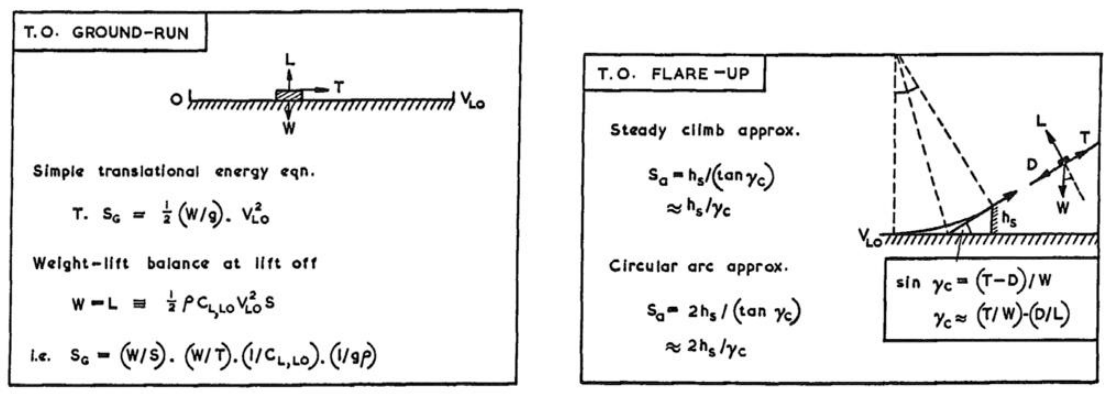
\includegraphics[width=0.75\linewidth]{figures/obert_takeoff.png}
    \caption{Obert's take-off distance estimation method}
    \label{fig:obert_verification}
\end{figure}

\subsection{Embry-Riddle}
An Embry-Riddle website provides another method with which the lift-off distance can be approximated\footnote{\url{https://eaglepubs.erau.edu/introductiontoaerospaceflightvehicles/chapter/takeoff-landing-performance/}} with the following equation: 

\begin{equation}\label{eq:s_LO}
    s_{LO} = \frac{1.44 \cdot W^2}{g \cdot \rho S C_{L,max}T},
\end{equation}

with $T$ as the average thrust: $T_{ave} = \frac{T_\text{static}+T_\text{max}}{2}$, determined according to Equation~\eqref{eq:thrust_levelII}.

\subsection{Torenbeek}
Torenbeek's first method is cumbersome and requires some assumptions. The take-off distance is split up into a ground phase and rotation phase: $s_{to} = s_{0-R}+s_R$. The following equations describe $s_{0-R}$ and $s_R$;

\begin{equation}\label{eq:distance_zero_rotate}
    s_{0-R} = \frac{V_x^2}{2g(\Bar{T}/W-\mu)}\cdot \frac{1}{a}\ln{\frac{1}{1-a}},
\end{equation}
with
\begin{equation}\label{eq:torenbeek_a}
    a = \frac{C_{D_G}-\mu C_{L_G}}{1.13C_{L_{max}} (\Bar{T}/W-\mu)}\left(\frac{V_x}{V_s}\right)^2,
\end{equation}
and
\begin{equation}\label{eq:torenbeek_a}
    s_R = 0.5 (V_R+V_{LOF}) \frac{\alpha_{LOF}-\alpha_G}{(d\theta/dt)_R},
\end{equation}
with
\begin{equation}\label{eq:torenbeek_a}
    V_{LOF} = V_R + g \left(\frac{T-D}{W}\right)_{LOF}  \frac{\alpha_{LOF}-\alpha_G}{(d\theta/dt)_R}.
\end{equation}

For $\alpha_{lof}$ you can assume a value or use the long equation 10-10 from Torenbeek~\cite{torenbeek2013synthesis} as given in his book.

\subsection{Torenbeek 2}
Torenbeek's latest book~\cite{torenbeek2013advanced} gives a simplified equation for the take-off distance, still considering two flight phases. However, Torenbeek added a term to account for engine failure in this equation:

\begin{equation}\label{eq:Torenbeek2}
    s_{TO} = \frac{W_{TO}^2}{\rho_{TO} g S_W C_{L_2} k_T T_{V_2}} + h_{TO}\cdot \left(\frac{(1-N_{eng}^{-1})T_{V_2}}{W_{TO}} - \left(C_0 + \frac{C_{L_2}}{\pi A_w e}\right) \right)^{-1},
\end{equation}

with $k_T=0.85$, $h_{TO}$ as the screen height (35ft) and $C_0=0.025$ to account for parasitic drag.

\subsection{Roskam}
Roskam's method is based on statistics of CS23 (smaller) aircraft. The equation is as follows:

\begin{equation}\label{eq:Roskam}
    s_{TO} = 1.66 \cdot (4.9 \cdot TOP + 0.09 \cdot TOP^2),
\end{equation}
with
\begin{equation}\label{eq:Roskam_TOP}
    TOP=\frac{(W/S)_{TO}(W/P)_{TO}}{\sigma C_{L_{max,TO}}},
\end{equation}
with $\sigma$ being the ratio of air density at the airport versus air density at sea-level. Although this equation probably works well for smaller aircraft, it is inaccurate for larger propeller aircraft. This is shown in \autoref{fig:roskam_inaccuracy}, where you can clearly see that most turboprop aircraft fall outside Roskam's data region in terms of $TOP$.

\begin{figure}[!ht]
    \centering
    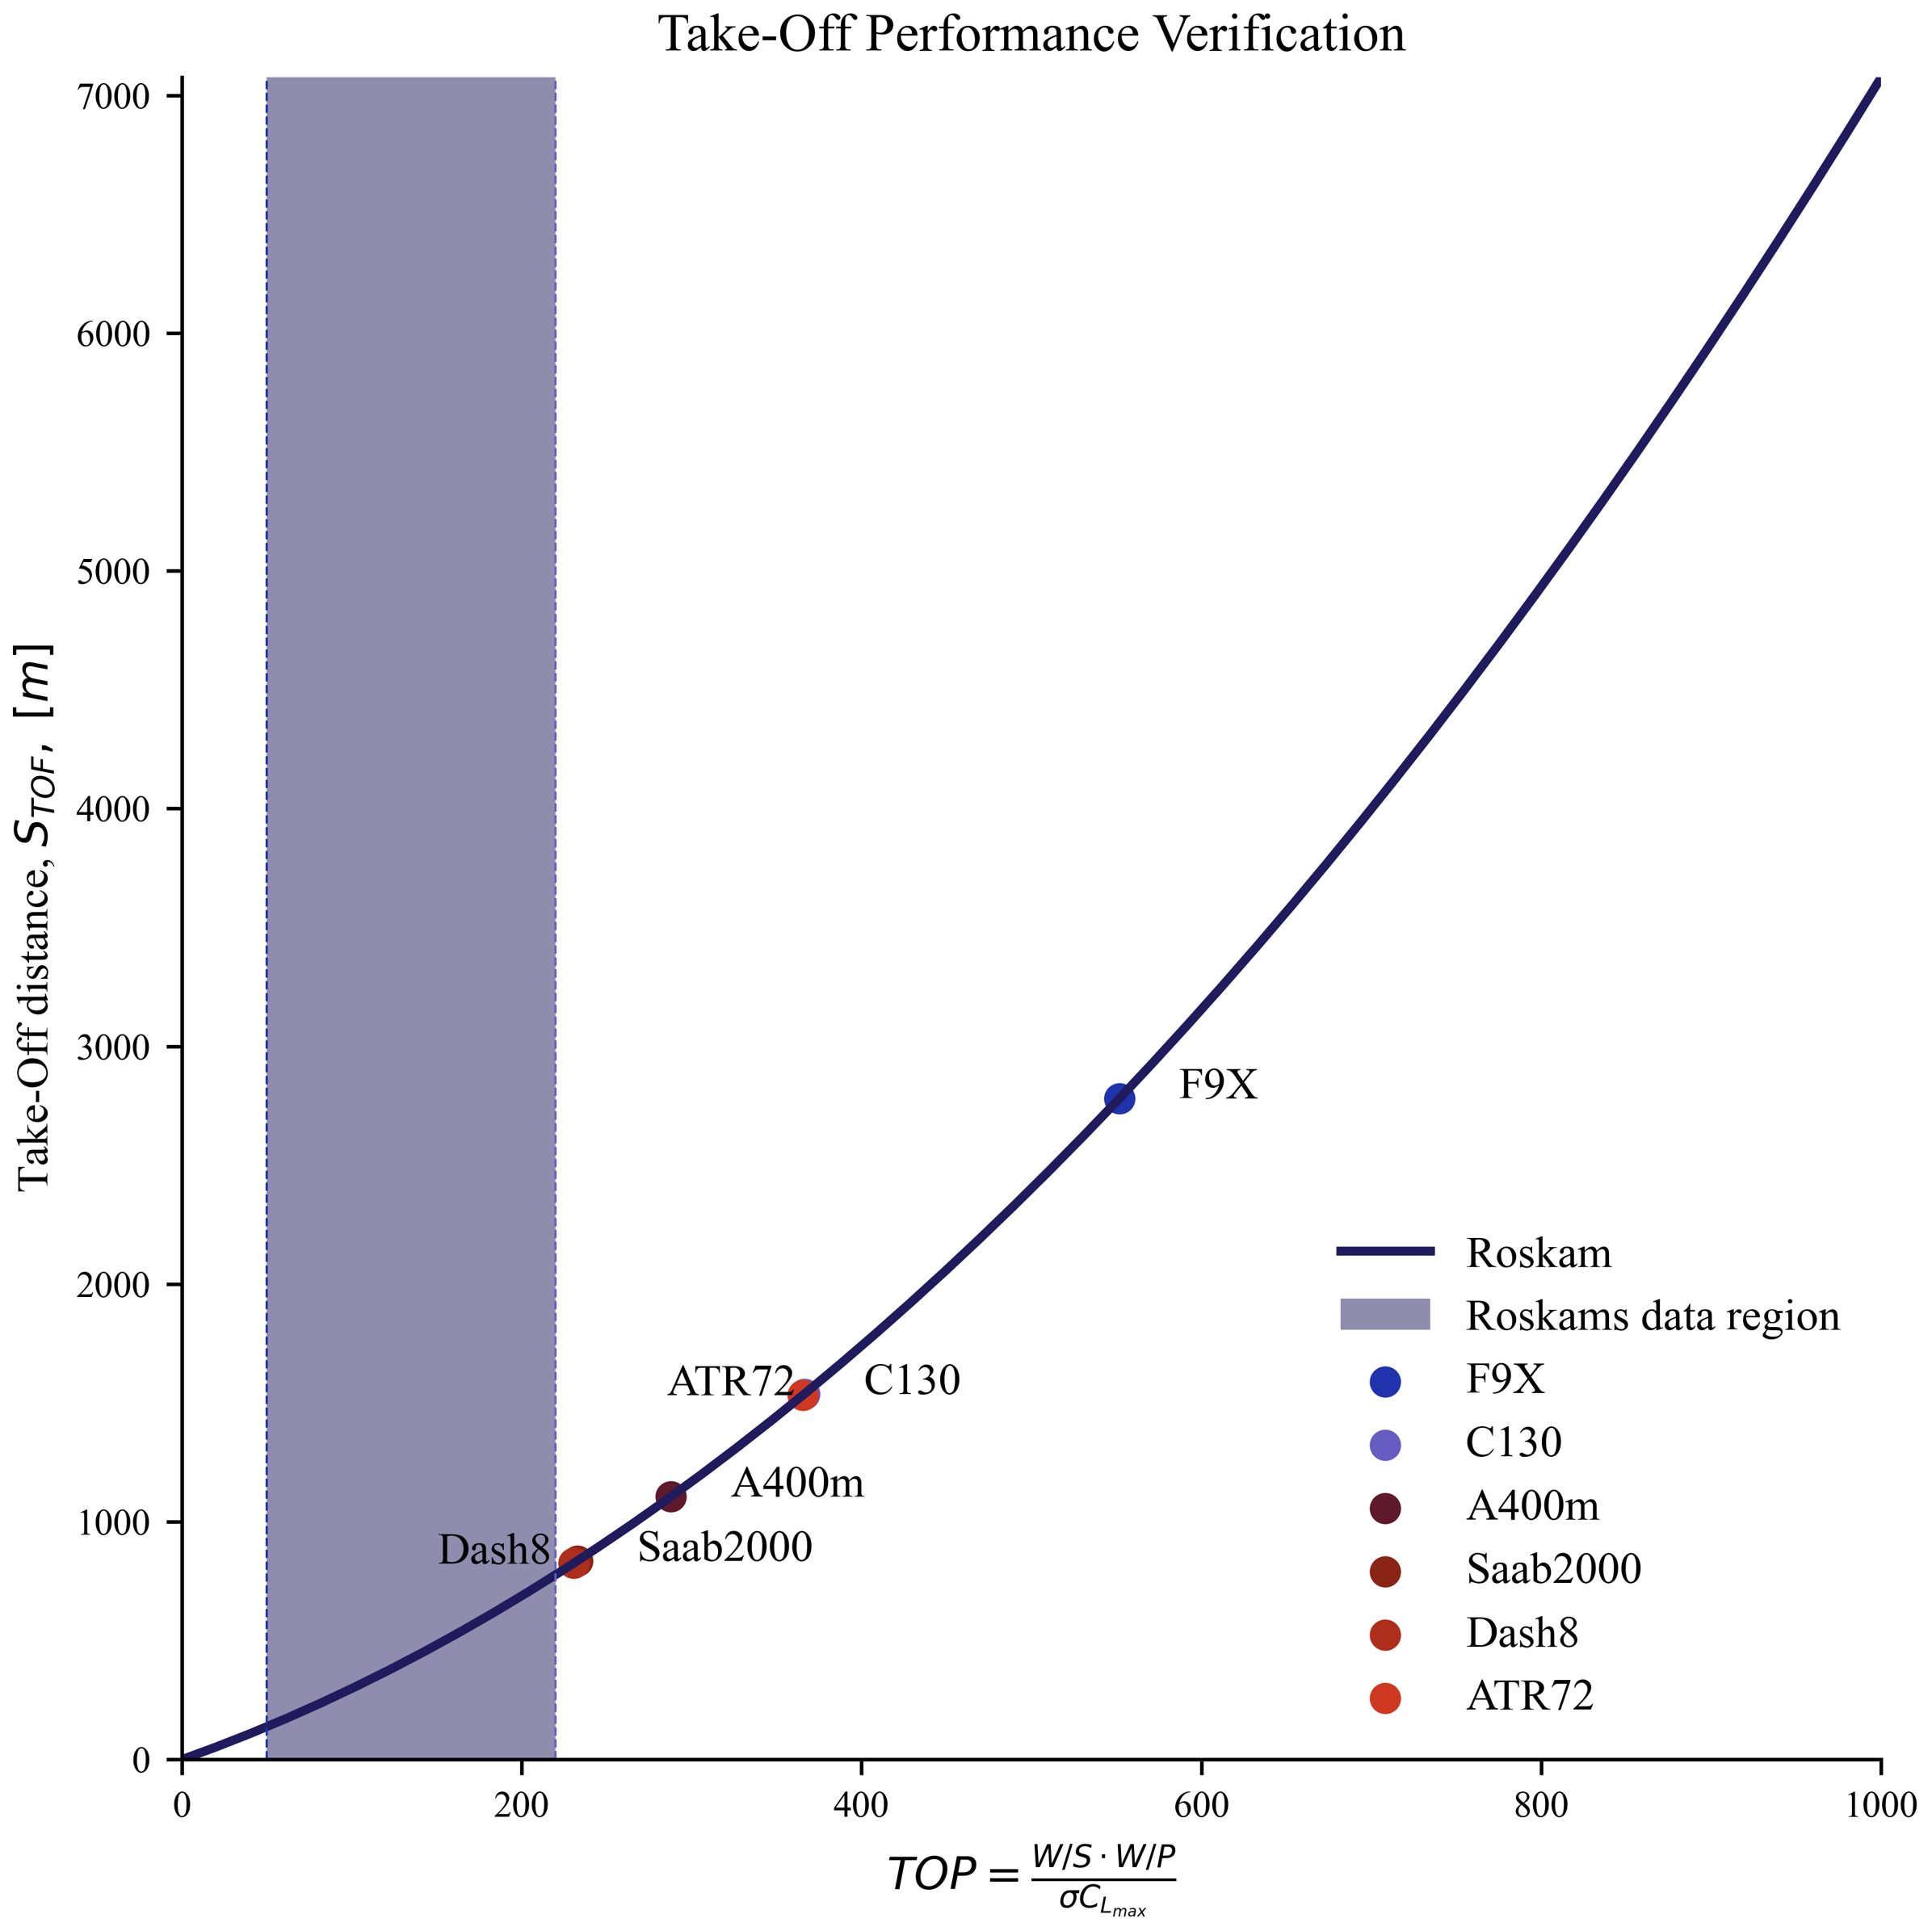
\includegraphics[width=0.5\linewidth]{figures/roskam_inaccurate.png}
    \caption{Visualisation of region where Roskam's equation holds}
    \label{fig:roskam_inaccuracy}
\end{figure}

\subsection{Raymer}
Raymer formulated a comparable equation to Roskam's work, but used a different data set, making it more suitable for the large turboprop class.

\begin{equation}\label{eq:raymer_TOP}
    TOP = ((W)/S_{ref})/((N_{eng} \cdot P)/W \cdot C_{L_{TO,max}})
\end{equation}

\begin{equation}\label{eq:raymer}
    s_{TO} = (TOP-6.217443298)/0.084958084
\end{equation}

\subsection{Mihaela}
Mihaela Nita was a bachelor student who worked out the take-off performance for the ATR72, and with that work gives an effective summary of the equations required. In her take-off equation she replaces $T$ with $T=\eta P /V$, given the following equation:

\begin{equation}\label{eq:mihaela}
    \frac{P_s/m_{MTO}}{m_{MTO}/S_w} \geq \frac{k_{TO}1.2\cdot V_{s,1}g}{s_{TOFL}\sigma C_{L,max,TO}\eta_p\sqrt{2}}
\end{equation}

\section{Validation}\label{sec:validation}
Validation is the process of comparing numerical results to experimental results and is the second step in checking whether the numerical model is correct. In the previous section we discussed verification equations. In this section the validation aircraft are given. The individual properties of each aircraft have been retrieved using FCOMs and can be found in the \texttt{examples/example\_classes} folder in the code repository. The following aircraft have been chosen for the validation process: ATR42, ATR72, Fokker 50, Dash8-300 and the KingAir.

\section{Results}\label{sec:VVresults}
The results of the verification and validation are shown in \autoref{fig:VV}. The verification process shows that the numerical model and several other theoretical models shows consistent and good similarity. It is expected that the power based methods with multiple take-off phases perform best. This hypothesis is verified since the Torenbeek 2 method and the numerical model consistently predict the approximate same take-off distance. Furthermore, as expected, the Roskam method is completely erroneous, where Raymer's statistical model shows good similarity with the numerical model.

The validation data was retrieved from FCOMs, which is experimental flown data. For some aircraft it also appeared hard to find accurate performance metrics. Some aircraft, such as the ATR42 and ATR72 -- for which it was easy to find data -- the numerical model shows good similarity. For other aircraft -- for which it proved to be hard to retrieve data -- the numerical model performs worse. Small inaccuracies in $C_L$ performance can have a huge impact on the take-off performance, thus it is expected that ambiguity around these factors introduces a significant error.

\begin{figure}[!ht]
    \centering
    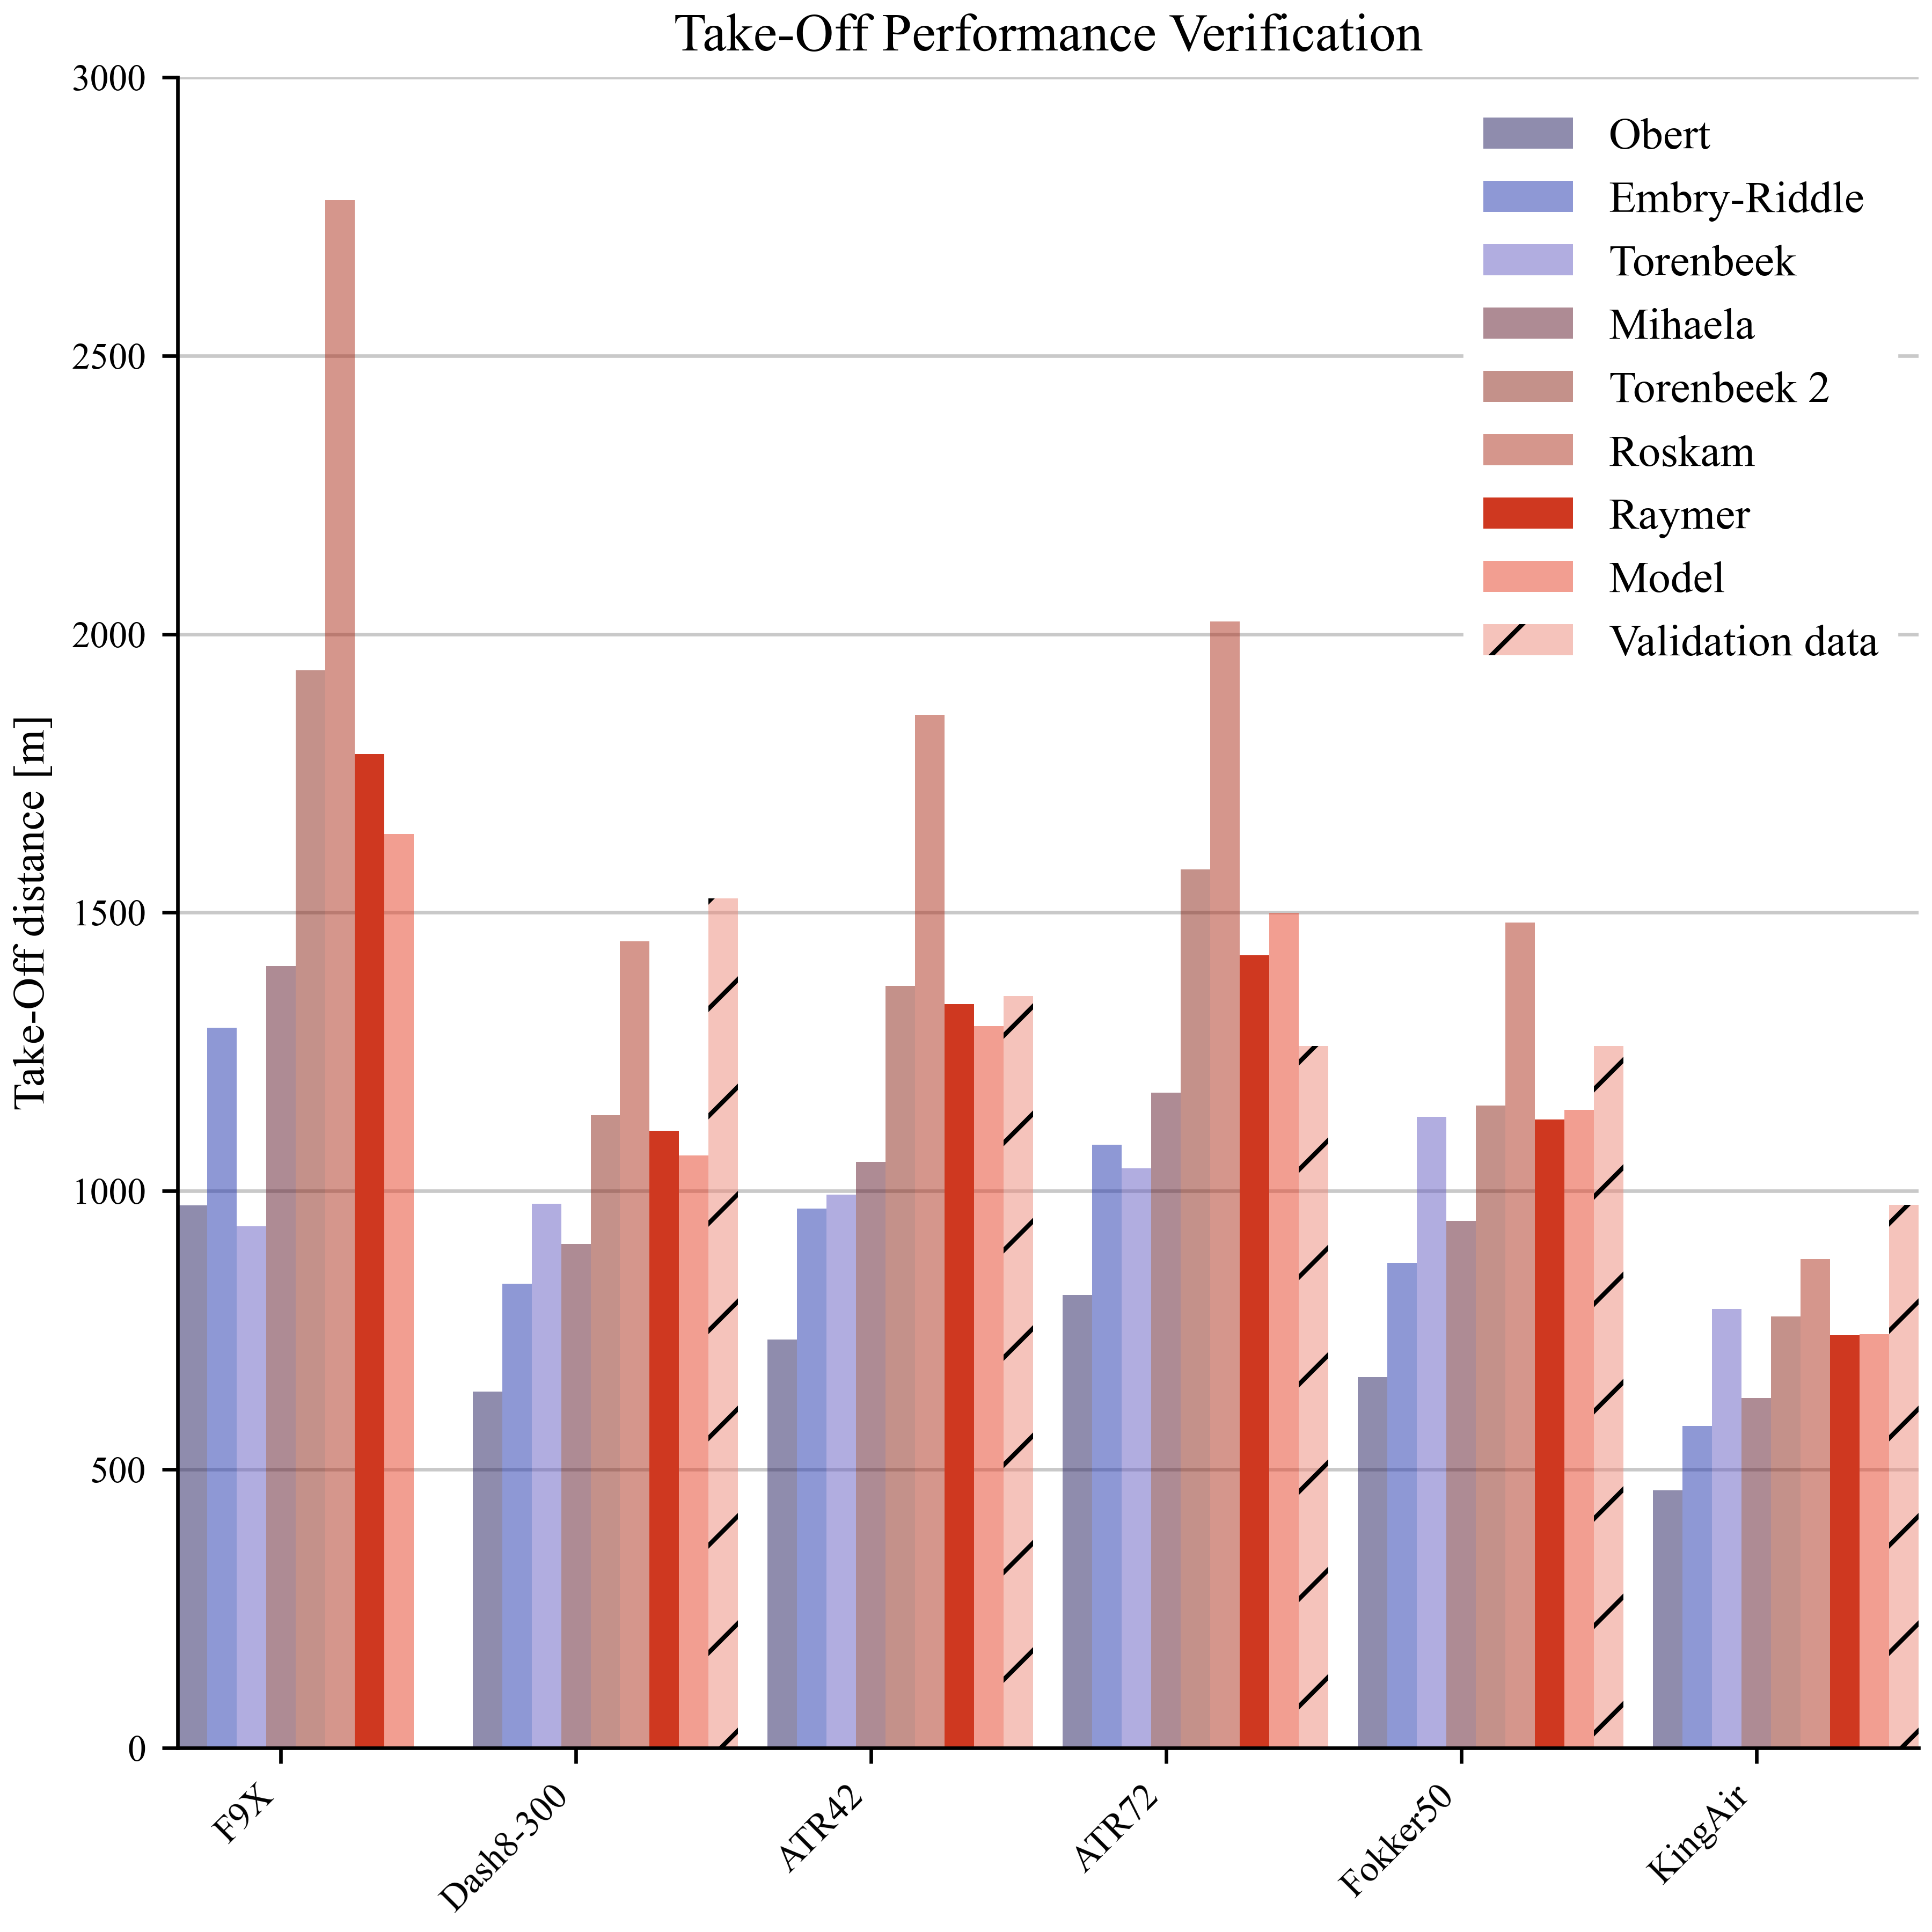
\includegraphics[width=0.5\linewidth]{figures/VERIFICATION.png}
    \caption{Verification and validation results of the numerical model}
    \label{fig:VV}
\end{figure}

Furthermore, the one engine inoperative (OEI) scenario should be verified as well. No experimental data exists about tis scenario so validation of the model cannot be performed. The verification procedure only uses the method described in the second book of Torenbeek~\cite{torenbeek2013advanced}, since it gives the option to model the system with one engine inoperative. The numerical model and the verification method show good resemblance as shown in \autoref{fig::verification_OEI}, with only a small disparity, likely due to the rotation strategy that isn't incorporated in Torenbeek's model. 

\begin{figure}[!ht]
    \centering
    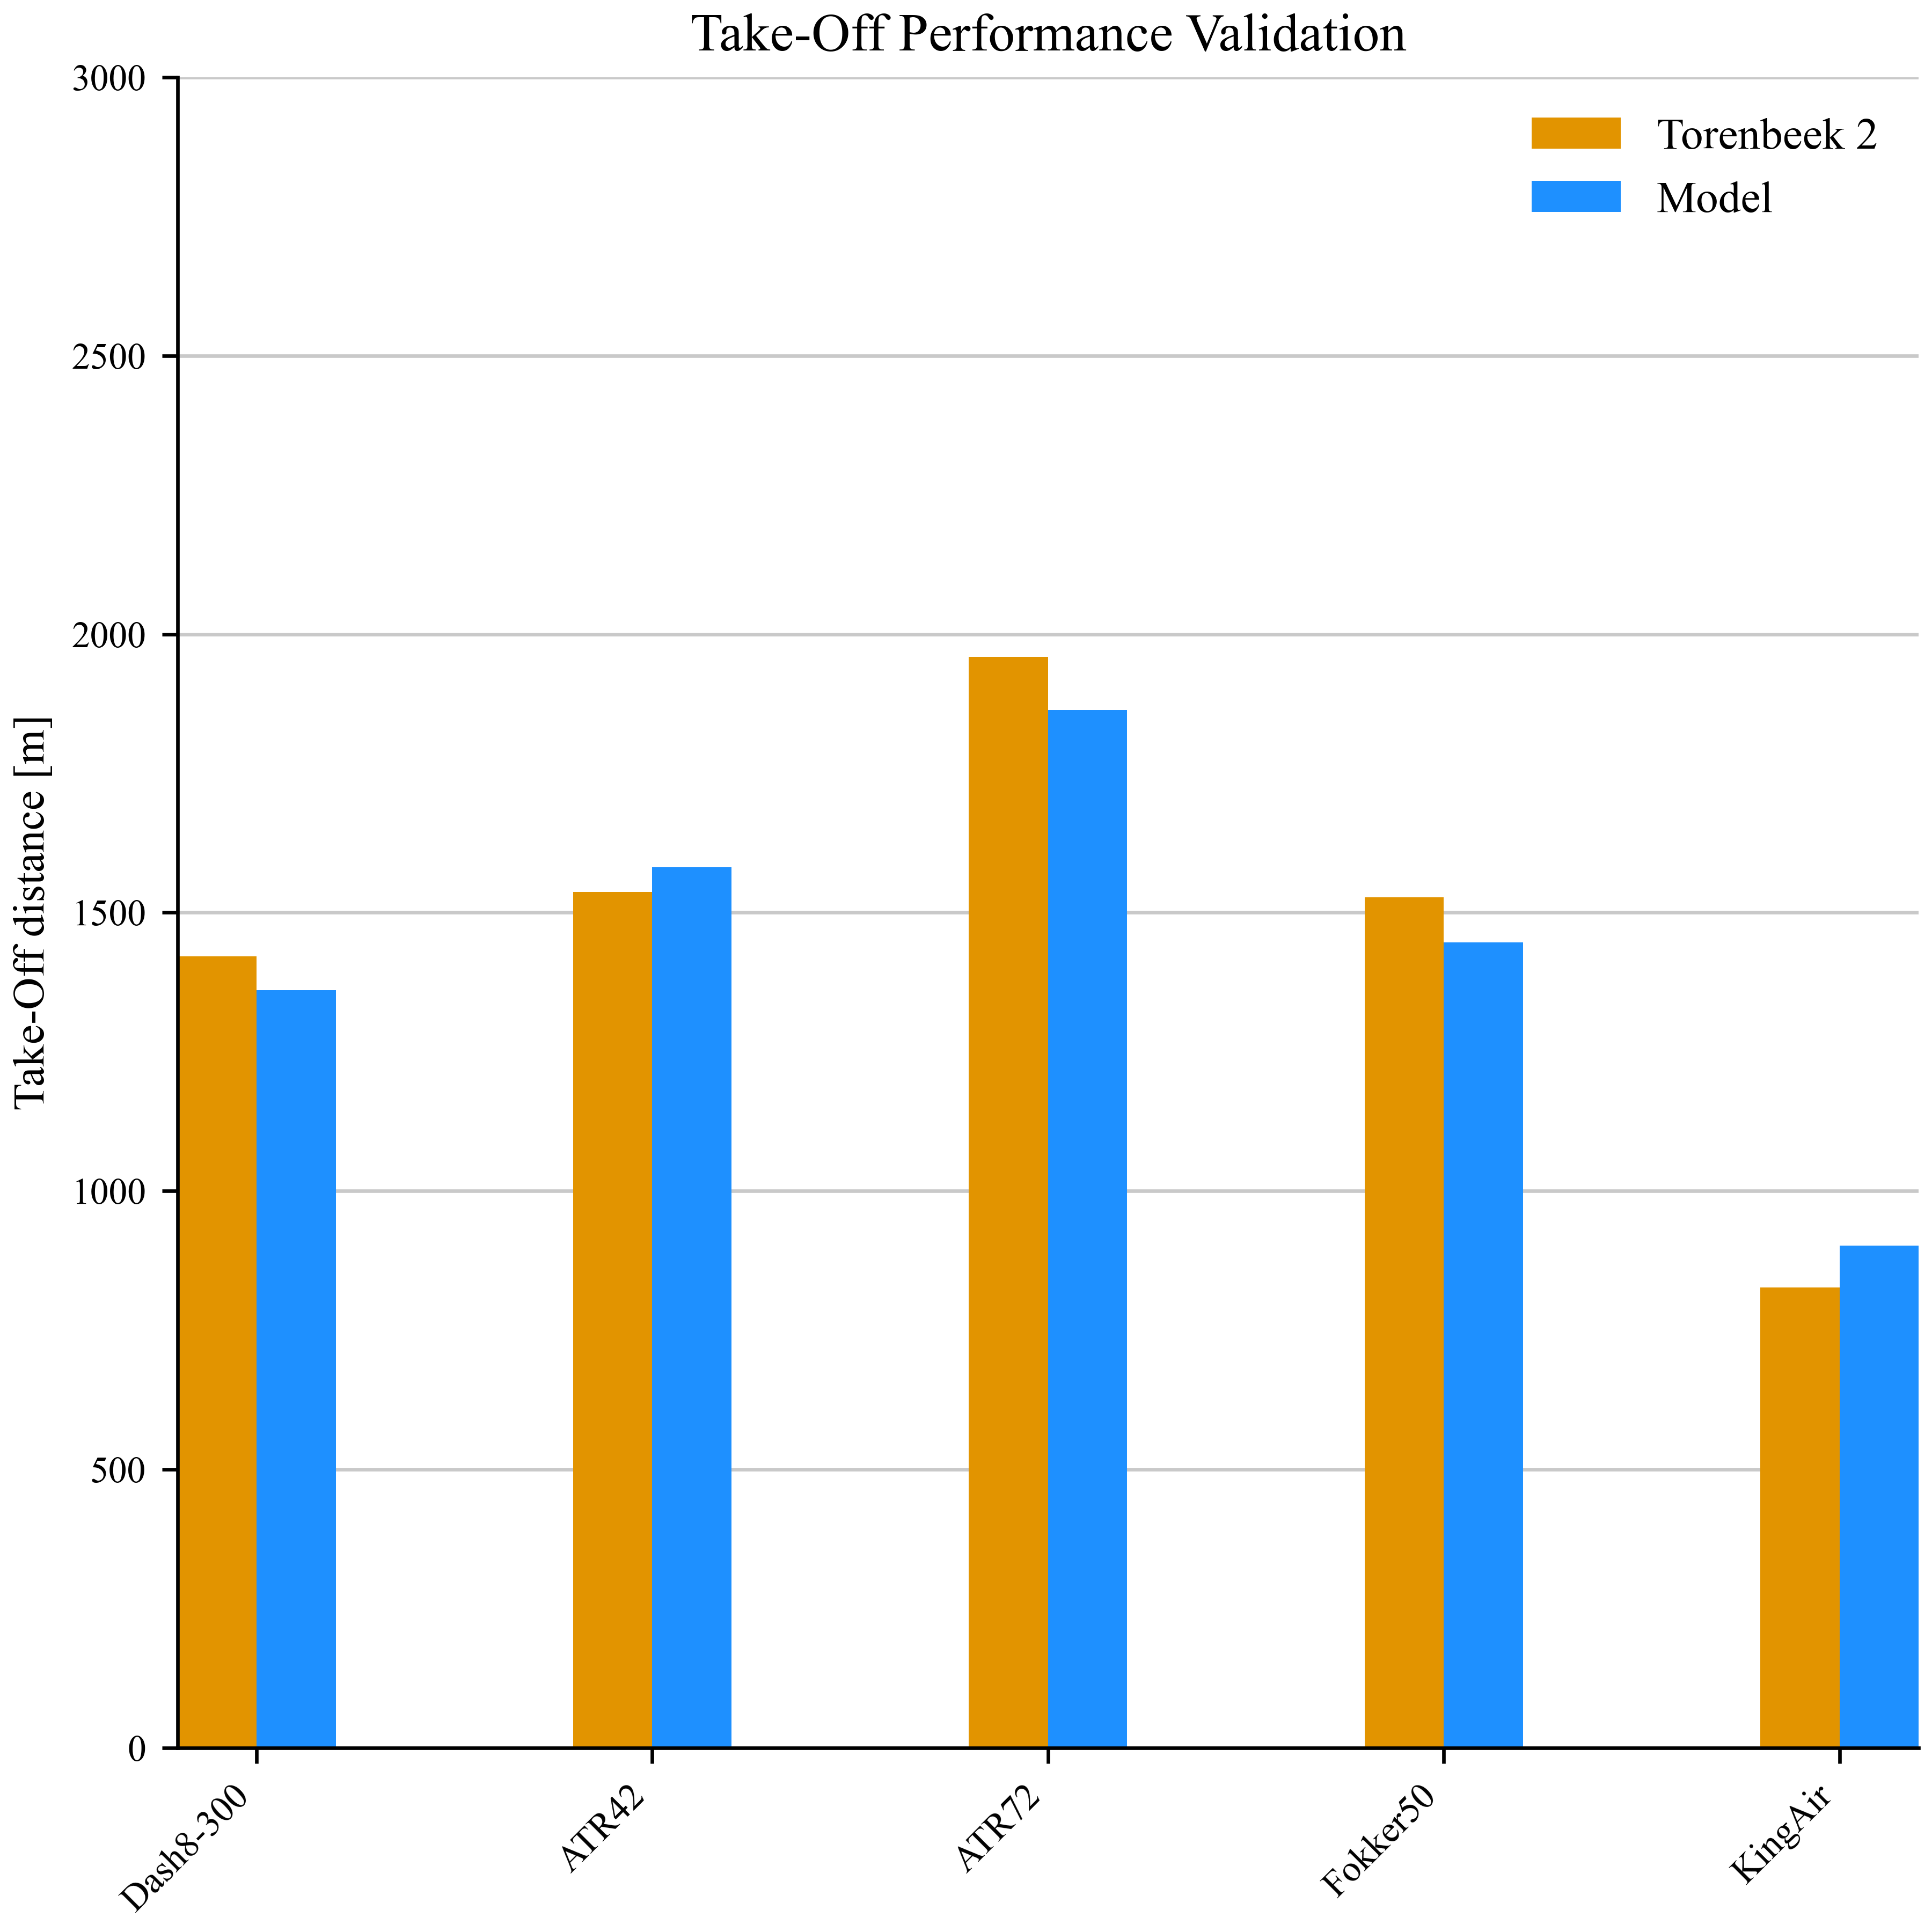
\includegraphics[width=0.5\linewidth]{figures/VALIDATION_OEI.png}
    \caption{Verification and validation results of the numerical model}
    \label{fig:verification_OEI}
\end{figure}

All in all, it can be concluded that the model performs decently well and generally returns the same results at the chosen verification methods and validation data. Therefore, it can be stated that the model returns decently accurate results.